%%% Třetí kapitola

\chapter{Testování algoritmu na datech}

V této sekci představíme výsledky implementace výpočtu Jonesova polynomu. Změříme délku běhu algoritmu a jeho variant na malých uzlech, náhodých uzlech a lincích a na speciálních typech uzlů.

\section{Malé tabulkové uzly}

Prostě že se to dělá a že to je rychlé a že je ta tabulka. Větší smysl to má pro větší.
\section{Náhodné uzly a linky}

\subsection{Generování náhodných linků a uzlů}
Náhodné linky budeme generovat pomocí rovinných grafů, neboť mezi linky a rovinnými grafy existuje vzájemně jednoznačná korespondence, zdroj?. (Jedná se o jinou korespondenci,  než tu mezi linky a rovinnými grafy s vrcholu stupně čtyři popsanou v sekci **).

\subsubsection{Převod rovinného grafu na link}
Rovinný graf z $n$ hranami odpovídá linku s $n$ kříženími. Každé hraně přířadíme náhodně kladné, či záporné znamení a umístíme na ni křížení příslušného typu. Úseky mezi kříženími jsou tím již jednoznačně určené: musí spojovat křížení mezi nejbližšími hranami tak, aby nevznikla žádná další křížení.

OBRÁZEK, KRESLENÝ RUKOU

\subsubsection{Generování náhodných rovinných grafů}
Graf s $n$ hranami získáme následujícím způsobem. Vygenerujeme vhodný počet náhodných bodů v rovině a nalezeneme jejich triangulaci, tj. spojíme body hranami tak, aby byl polygon tvořící konvexní obal bodů rozdělen na trojúhelníky.

\begin{figure}[h]  
\centering 
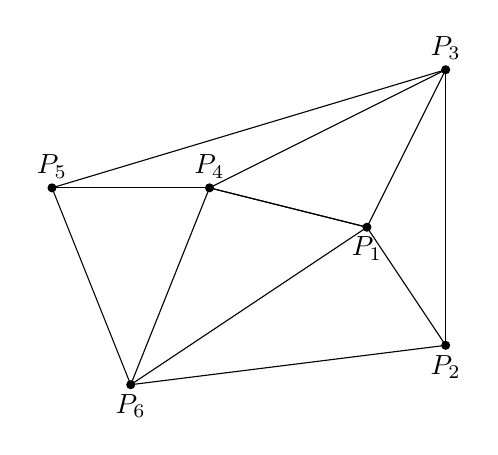
\begin{tikzpicture}
\draw[fill] (1,1) circle [radius=0.05];
\node [below] at (1,1) {$P_1$};

\draw[fill] (2,-1/2) circle [radius=0.05];
\node [below] at (2,-1/2) {$P_2$};

\draw[fill] (2,3) circle [radius=0.05];
\node [above] at (2,3) {$P_3$};

\draw[fill] (-1,3/2) circle [radius=0.05];
\node [above] at (-1,3/2) {$P_4$};

\draw[fill] (-3,3/2) circle [radius=0.05];
\node [above] at (-3,3/2) {$P_5$};

\draw[fill] (-2,-1) circle [radius=0.05];
\node [below] at (-2,-1) {$P_6$};

\draw (-3,3/2) -- (2,3);
\draw (-3,3/2) -- (-1,3/2);
\draw (-3,3/2) -- (-2,-1);
\draw (-1,3/2)  -- (2,3) ;
\draw (-1,3/2)  -- (-2,-1) ;
\draw (-1,3/2)  -- (1,1) ;
\draw (-1,3/2)  -- (1,1) ;
\draw (2,3)   -- (1,1) ;
\draw (-2,-1) -- (1,1) ;
\draw (-2,-1) -- (2,-1/2);
\draw  (1,1)  -- (2,-1/2);
\draw  (2,3)-- (2,-1/2);
\end{tikzpicture}
\caption{Triangulace šesti bodů}
\end{figure}  

Získali jsme tak rovinný graf s původními body jako vrcholy. Pokud je počet hran menší než $n$, provedeme triangulaci znovu s větším počtem bodů. Pokud je počet hran větší než $n$, odstraníme potřebný počet náhodně zvolených hran.

\subsubsection{Implementace}

Triangulace bodů je snadno implementovatelný geometrický problém. \\ Se získaným rovinným grafem pracujeme jako s množinou vrcholů a k nim příslušným hranám seřazeným v pořadí, jak k danému vrcholu přiléhají. Z této struktury je již možné získat PD notaci příslušného linku.


V PD notaci lze procházkou po vláknu snadno poznat, jestli je vygenerovaný link uzlem. Také jsme v PD notaci jednoduchou operací schopni uzel změnit na alternující, tedy takový, v němž se střídají křížení vedená zespodu a zvrchu.

Jsme tedy schopni nagenerovat uzly, alternující uzly a linky libovolné velikosti.

Takto generované uzly jsou také poměrně \uv{zamotané}, tedy rozmotávací krok algoritmu neodstraní příliš mnoho křížení.

\subsection{Test}
Rozdíl mezi uzly a alternujícími uzly.
Rozdíly algoritmů na uzlech.
Linky?
U uzlů a alt od větších uzlů fitovat data a shrnout.

\section{Torusové uzly}
Rovnou srovnání B a R.

Pak rozebrat ty dva kusy.

Nezapomenou dělat závěry a shrnovat.

